% Paquets généraux
\documentclass[a4paper,12pt,titlepage]{article}
\usepackage[T1]{fontenc}
\usepackage[utf8]{inputenc}
\usepackage[french]{babel}
\usepackage[gen]{eurosym}
%\usepackage[dvips]{graphicx}
\usepackage{fancyhdr}
\usepackage{pdfpages} 
\usepackage{multido}
\usepackage{moreverb}
\usepackage{hyperref}
%\usepackage{textcomp}
\usepackage{verbatim}
\usepackage{moreverb}
\usepackage{listings}
\usepackage{minted}
\usepackage{eso-pic}
\usepackage{enumitem}
\usepackage{comment}
\usepackage{boxedminipage}
\usepackage[french,onelanguage, boxruled,linesnumbered]{algorithm2e}


\newcommand{\auteurun}{Juliette Genzmer}
\newcommand{\auteurdeux}{Willie Robert}
\newcommand{\auteurtrois}{Renaud Costadoat}
\newcommand{\institute}{Lycée Dorian}
\newtheorem{solution}{Solution}


\newcommand{\nom}{Le labyrinthe}
\newcommand{\sequence}{1}
\newcommand{\numero}{04}
\newcommand{\type}{DS}
\newcommand{\descrip}{Le labyrinthe}


\usepackage{color}
\usepackage{xcolor}
\usepackage{colortbl}
\usepackage{helvet}
\renewcommand{\familydefault}{\sfdefault}
\usepackage{amsfonts}
\usepackage{amsmath}
%\usepackage{xspace}
\usepackage{varioref}
\usepackage{tabularx}
%\usepackage{floatflt}
\usepackage{graphics}
\usepackage{wrapfig}
\usepackage{textcomp}
\usepackage{tikz}
\usepackage{wrapfig}
\usepackage{gensymb}
\usepackage{ifthen}
\usepackage{cancel}
\usepackage{etoolbox}
\usepackage{multirow}
%\usepackage{boxedminipage}
\definecolor{gris25}{gray}{0.75}
\definecolor{bleu}{RGB}{18,33,98}
\definecolor{bleuf}{RGB}{42,94,171}
\definecolor{bleuc}{RGB}{231,239,247}
\definecolor{rougef}{RGB}{185,18,27}
\definecolor{rougec}{RGB}{255,188,204}%255,230,231
\definecolor{vertf}{RGB}{103,126,82}
\definecolor{vertc}{RGB}{220,255,191}
\definecolor{forestgreen}{rgb}{0.13,0.54,0.13}
\definecolor{blcr}{rgb}{0.59,0.69,0.84}
\definecolor{blfr}{rgb}{0.32,0.51,0.75}
\definecolor{orfr}{rgb}{0.90,0.42,0.15}
\definecolor{orcr}{rgb}{0.90,0.65,0.50}
\definecolor{orangef}{rgb}{0.659,0.269,0.072}
\definecolor{orange}{rgb}{0.58,0.35,0.063}
\definecolor{orangec}{rgb}{0.43,0.32,0.25}
\definecolor{rcorrect}{rgb}{0.6,0,0}
\definecolor{sequence}{rgb}{0.75,0.75,0.75}
\definecolor{competences}{rgb}{0.61,0.73,0.35}
\definecolor{grisf}{HTML}{222222}
\definecolor{grisc}{HTML}{636363}
\definecolor{normal}{HTML}{4087c4}
\definecolor{info}{HTML}{5bc0de}
\definecolor{success}{RGB}{92,184,92}
\definecolor{warning}{RGB}{240,173,78}
\definecolor{danger}{RGB}{217,83,79}
\hypersetup{                    % parametrage des hyperliens
    colorlinks=true,                % colorise les liens
    breaklinks=true,                % permet les retours à la ligne pour les liens trop longs
    urlcolor= blfr,                 % couleur des hyperliens
    linkcolor= orange,                % couleur des liens internes aux documents (index, figures, tableaux, equations,...)
    citecolor= forestgreen                % couleur des liens vers les references bibliographiques
    }

% Mise en page
\pagestyle{fancy}

\setlength{\hoffset}{-18pt}

\setlength{\oddsidemargin}{0pt} 	% Marge gauche sur pages impaires
\setlength{\evensidemargin}{0pt} 	% Marge gauche sur pages paires
\setlength{\marginparwidth}{00pt} 	% Largeur de note dans la marge
\setlength{\headwidth}{481pt} 	 	% Largeur de la zone de tête (17cm)
\setlength{\textwidth}{481pt} 	 	% Largeur de la zone de texte (17cm)
\setlength{\voffset}{-18pt} 		% Bon pour DOS
\setlength{\marginparsep}{7pt}	 	% Séparation de la marge
\setlength{\topmargin}{-30pt} 		% Pas de marge en haut
\setlength{\headheight}{55pt} 		% Haut de page
\setlength{\headsep}{20pt} 		% Entre le haut de page et le texte
\setlength{\footskip}{30pt} 		% Bas de page + séparation
\setlength{\textheight}{700pt} 		% Hauteur de l'icone zone de texte (25cm)
\setlength\fboxrule{1 pt}
\renewcommand{\baselinestretch}{1}
\setcounter{tocdepth}{1}
\newcommand{\cadre}[2]
{\fbox{
  \begin{minipage}{#1\linewidth}
   \begin{center}
    #2\\
   \end{center}
  \end{minipage}
 }
}

\newcounter{num_quest} \setcounter{num_quest}{0}
\newcounter{num_rep} \setcounter{num_rep}{0}
\newcounter{num_cor} \setcounter{num_cor}{0}

\newcommand{\question}[1]{\refstepcounter{num_quest}\par
~\ \\ \parbox[t][][t]{0.15\linewidth}{\textbf{Question \arabic{num_quest}}}\parbox[t][][t]{0.85\linewidth}{#1\label{q\the\value{num_quest}}}\par\par
}



\newcommand{\reponse}[0]{\refstepcounter{num_rep}\par
~\ \\ \parbox[t][][t]{0.15\linewidth}{\textbf{Question \arabic{num_rep}}}}

\newcommand{\cor}
{\refstepcounter{num_cor}
\noindent
\rule{\linewidth}{.5pt}
\textbf{Question \arabic{num_cor}:} \\
}



% En tête et pied de page
\lhead{\nom}
\rhead{
\includegraphics[width=2cm]{../../../img/logo}}
\lfoot{David Aubert, Renaud Costadoat}
\rfoot{Page \thepage}
\cfoot{}

\newlength{\RoundedBoxWidth}
\newsavebox{\GrayRoundedBox}
\newenvironment{GrayBox}[1][\dimexpr\textwidth-4.5ex]%
   {\setlength{\RoundedBoxWidth}{\dimexpr#1}
    \begin{lrbox}{\GrayRoundedBox}
       \begin{minipage}{\RoundedBoxWidth}}%
   {   \end{minipage}
    \end{lrbox}
    \begin{center}
    \begin{tikzpicture}%
       \draw node[draw=bleuf,fill=bleuc,rounded corners,%
             inner sep=2ex,text width=\RoundedBoxWidth]%
             {\usebox{\GrayRoundedBox}};
    \end{tikzpicture}
    \end{center}}

\fancypagestyle{correction}{%
  \fancyhf{}
  \lhead{\colorbox{danger}{\begin{minipage}{0.65\paperwidth} \textcolor{white}{\textbf{Correction}} \end{minipage}} }
  \rhead{
\includegraphics[width=2cm]{../../../img/logo}}
  \lfoot{Juliette Genzmer, Willie Robert, Renaud Costadoat}
  \rfoot{\colorbox{danger}{\begin{minipage}{0.3\paperwidth} \begin{flushright}\textcolor{white}{\textbf{Correction}}\end{flushright} \end{minipage}} }}

\renewcommand{\footrulewidth}{0.4pt}


\newcommand{\BackgroundPic}{%
\put(0,0){%
\parbox[b][\paperheight]{\paperwidth}{%
\vfill
\begin{center}
\hspace{0.5cm}\vspace{0.5cm}

\includegraphics[width=\paperwidth,height=\paperheight,%
keepaspectratio]{../../../img/fond5}%
\end{center}
\vfill
}}}

\newcommand{\goforum}{
\begin{figure}[ht!]
\begin{center}
 
\includegraphics[width=0.7\linewidth]{../../../img/go_forum}
\end{center}
\label{go_forum}
\caption{J'pète les plombs}
\end{figure}}

\newcommand{\BackgroundPicdeux}{%
\put(25,-30){%
\parbox[b][\paperheight]{\paperwidth}{%
\vfill
\begin{center}

\includegraphics[width=\paperwidth,height=\paperheight,%
keepaspectratio]{../../../img/fond6}%
\end{center}
\vfill
}}}

\setenumerate[1]{align=left,label=\arabic*}
\setenumerate[2]{before=\stepcounter{enumi},label*=.\arabic*,leftmargin=1.2em,align=left}

\begin{document}


\pagestyle{fancy}

\AddToShipoutPicture{\BackgroundPicdeux}

\begin{center}
{\Large\bf {\type} \no {\numero} -- \descrip}
\end{center}

\SetKw{KwFrom}{de} 

\begin{boxedminipage}{.9\textwidth} 
\begin{itemize}
 \item Faire tous les exercices dans un fichier {NomPrenom.py} à sauvegarder,
 \item mettre en commentaire l'exercice et la question traités (ex: \# Exercice 1),
 \item ne pas oublier pas de commenter ce qui est fait dans votre code (ex: \# Je crée une fonction pour calculer la racine d'un nombre),
 \item il est possible de demander un déblocage pour une question, mais celle-ci sera notée 0,
 \item il faut vérifier avant de partir que le code peut s'exécuter et qu'il affiche les résultats que vous attendez. Les lignes de code qui doivent s'exécuter sont décommentées.
\end{itemize}
\end{boxedminipage}

\section*{Contexte et cadre général}

On cherche à résoudre un labyrinthe, figure \ref{fig01}, représenté sous forme d'une \textbf{grille de $14 \times 20$ cases}.

Chaque case est soit un \textbf{mur} (en noir, valeur~\texttt{1}), soit une \textbf{case libre} (en blanc, valeur~\texttt{0}).

\begin{figure}[!ht]
	\begin{center}
		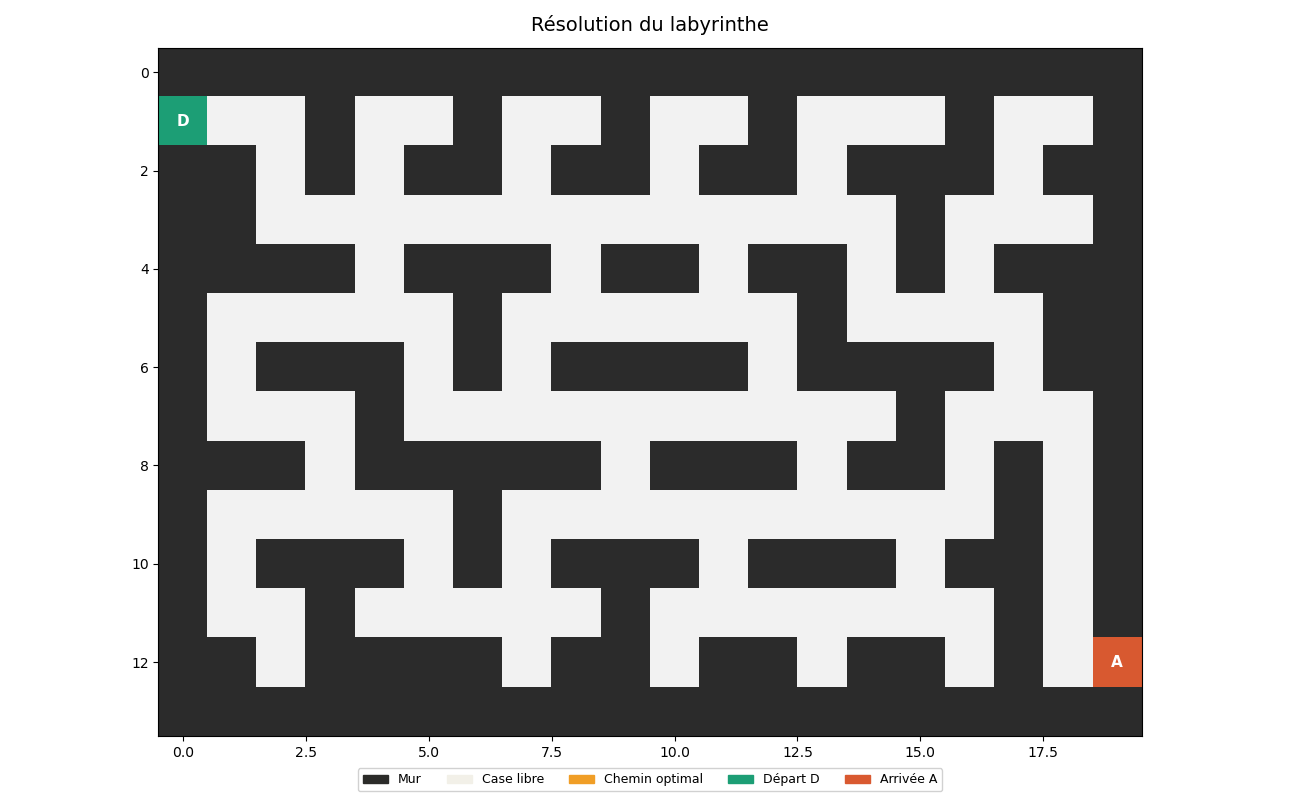
\includegraphics[width=0.9\linewidth]{img/labyrinthe_vide}
	\end{center}
	\caption{\label{fig01}Labyrinthe à résoudre}
\end{figure}

\begin{itemize}[leftmargin=1.5cm]
  \item Le \textbf{départ} $D$ est situé en \texttt{(ligne=1, col=0)}.
  \item L'\textbf{arrivée} $A$ est en \texttt{(ligne=12, col=19)}.
\end{itemize}

La grille est stockée dans un fichier CSV (\texttt{grille.csv}) où les cellules sont séparées par des \texttt{;} et chaque ligne correspond à une rangée du labyrinthe.

\medskip

Le squelette du programme (imports, constantes, fonction d'affichage \texttt{afficher}) vous est fourni dans un fichier \texttt{script\_candidat.py}. Vous devez le copier/coller à l'intérieur de votre fichier \texttt{NomPrenom.py}.

\section{Analyse du labyrinthe}

\subsection{Lecture du fichier CSV}

\question{\textbf{Écrire} le code permettant de lire le fichier \texttt{grille.csv} et de construire la variable \texttt{grille}, une liste de listes d'entiers (0 ou 1) représentant le labyrinthe. \textbf{Afficher} la première ligne (index=0) de \texttt{grille}.}

\subsection{Affichage initial du labyrinthe}

Pour faire la question suivante copier/coller le contenu du fichier \texttt{script\_candidat.py} dans votre script.

\question{\textbf{Appeler} la fonction \texttt{afficher()} pour afficher le labyrinthe.}

\subsection{Recherche des cases libres}

\question{\textbf{Écrire} le code qui construit la liste \texttt{cases\_libres} contenant toutes les cases de coordonnées $[i, j]$ telles que \texttt{grille[i][j] == 0}. \textbf{Afficher} la deuxième case (index=1) de \texttt{cases\_libres}.}

\subsection{Nommage des cases}

\question{\textbf{Écrire} la fonction \texttt{nom\_case(case)} qui, pour une case donnée sous forme de liste \texttt{[i, j]}, renvoie la chaîne de caractères \texttt{'[i,j]'}. \textbf{Afficher} \texttt{nom\_case([1, 2])} qui doit retourner \texttt{'[1,2]'}.}

\section{Parcours de graphe}

\subsection{Case suivante dans une direction}

On définit les quatre directions de déplacement :

\begin{minted}{python}
directions = [[0, 1], [0, -1], [1, 0], [-1, 0]]
\end{minted}

\question{\textbf{Écrire} la fonction \texttt{prochaine\_case(case, direction)} qui renvoie la case obtenue en appliquant le déplacement \texttt{direction} depuis \texttt{case}. \textbf{Afficher} \texttt{prochaine\_case([0, 1], directions[2])} qui doit retourner \texttt{[1, 1]}.}

\subsection{Construction du graphe}

\question{\textbf{Construire} le dictionnaire \texttt{graphe} tel que :
\begin{itemize}
  \item Chaque \textbf{clé} est le nom (chaîne de caractère) d'une case libre,
  \item La \textbf{valeur} associée est la liste des noms des cases libres adjacentes (haut, bas, gauche, droite) qui sont dans les limites de la grille.
\end{itemize}

\textit{Attention aux bords de la grille !}

\textbf{Afficher} \verb?graphe['[1,1]']? qui doit renvoyer \verb?['[1,2]', '[1,0]']?.}

\section{Résolution du labyrinthe}

\subsection{Recherche de tous les chemins}

La fonction \verb?tous_les_chemins(graphe, depart, arrivee)? permet de parcourir tous les chemins possible d'une case \verb?depart? à une case \verb?arrivee?.

\question{\textbf{Recopier} et compléter le code afin que la fonction renvoie les chemins attendus. Il n'est pas nécessaire de recopier les commentaires \texttt{\#}.}

\begin{minted}{python}
def tous_les_chemins(graph, depart, arrivee):

    chemins_a_explorer = [[depart]]
    resultats = []

    while len(chemins_a_explorer)>0:
        # Récupérer le premier chemin des chemins a explorer
        # Le supprimer des chemins a explorer
        chemin = chemins_a_explorer.pop(0)
        # Partir du dernier sommet de ce chemin
        ...................
        # Si on atteint l'arrivée
        if sommet == arrivee:
            # Stocker le chemin dans la liste resultats
            .......................
        else:
            # Pour chaque voisin de ce sommet
            for voisin in graph[sommet]:
                # On regarde si on est pas déjà passé par ce sommer
                if voisin not in chemin:
                    # On ajoute ce voisin à ce chemin
                    .................................
                    # On intègre ce chemin à la liste des chemins à explorer
                    .................................
    return resultats
\end{minted}

\subsection{Chemin le plus court}

\question{En utilisant le résultat de la fonction \texttt{tous\_les\_chemins}, \textbf{écrire} le code qui trouve le chemin de longueur minimale. \textbf{Appeler} la fonction \texttt{afficher(grille,chemin\_plus\_court)} qui affiche alors l'image du graphe avec le chemin le plus court en jaune.}

%  1 & Lecture CSV                         & 3 pts & E/S fichiers, listes \\
%  2 & Affichage initial                   & 1 pt  & Appel de fonction \\
%  3 & Recherche des cases libres          & 2 pts & Boucles imbriquées \\
%  4 & Fonction \texttt{nom\_case}         & 2 pts & Chaînes, fonctions \\
%  5 & Fonction \texttt{prochaine\_case}   & 2 pts & Fonctions, listes \\
%  6 & Construction du graphe             & 4 pts & Dictionnaires, structures \\
%  7 & Analyse \texttt{tous\_les\_chemins} & 4 pts & DFS, backtracking, analyse \\
%  8 & Chemin le plus court               & 3 pts & Algorithmes, min \\

\begin{center}
FIN
\end{center}
 
\cleardoublepage

\ifdef{\public}{\end{document}}{\pagestyle{correction}}

\begin{center}
\Large{Correction}
\end{center}

\reponse{}

\begin{minted}{python}
file = open('grille.csv', 'r')
contenu = file.read()
file.close()

lignes = contenu.split('\n')

grille = []
for ligne in lignes[:-1]:           # [:-1] ignore la derniere ligne vide
    data = [int(i) for i in ligne.split(';')]
    grille.append(data)
\end{minted}

\reponse{}

\begin{minted}{python}
afficher(grille, [])   # liste vide = aucun chemin a afficher
\end{minted}

\reponse{}

\begin{minted}{python}
cases_libres = []
for i in range(LIGNES):
    for j in range(COLS):
        if grille[i][j] == 0:
            cases_libres.append([i, j])
\end{minted}

\reponse{}

\begin{minted}{python}
def nom_case(case):
    return '[' + str(case[0]) + ',' + str(case[1]) + ']'
\end{minted}

\reponse{}

\begin{minted}{python}
directions = [[0, 1], [0, -1], [1, 0], [-1, 0]]

def prochaine_case(case, direction):
    return [case[0] + direction[0], case[1] + direction[1]]
\end{minted}

\reponse{}

\begin{minted}{python}
graphe = {}
for case_libre in cases_libres:
    graphe[nom_case(case_libre)] = []
    for direction in directions:
        prochaine = prochaine_case(case_libre, direction)
        # Verifier que la prochaine case est dans la grille
        if 0 <= prochaine[0] < LIGNES and 0 <= prochaine[1] < COLS:
            if grille[prochaine[0]][prochaine[1]] == 0:
                graphe[nom_case(case_libre)].append(nom_case(prochaine))
\end{minted}

\reponse{}

\begin{minted}{python}
def tous_les_chemins(graph, depart, arrivee):

    chemins_a_explorer = [[depart]]
    resultats = []

    while len(chemins_a_explorer)>0:
        # Récupérer le premier chemin des chemins a explorer
        # Le supprimer des chemins a explorer
        chemin = chemins_a_explorer.pop(0)
        # Partir du dernier sommet de ce chemin
        sommet = chemin[-1]
        # Si on atteint l'arrivée
        if sommet == arrivee:
            # Stocker le chemin dans la liste resultats
            resultats.append(chemin)
        else:
            # Pour chaque voisin de ce sommet
            for voisin in graph[sommet]:
                # On regarde si on est pas déjà passé par ce sommer
                if voisin not in chemin:
                    # On ajoute ce voisin à ce chemin
                    nouveau_chemin = chemin + [voisin]
                    # On intègre ce chemin à la liste des chemins à explorer
                    chemins_a_explorer.append(nouveau_chemin)
    return resultats

chemins = list(tous_les_chemins(graphe, nom_case(DEPART), nom_case(ARRIVEE)))
\end{minted}

\reponse{}

\begin{minted}{python}
chemin_plus_court = chemins[0]
for c in chemins:
    if len(c) < len(chemin_plus_court):
        chemin_plus_court = c

print(' -> '.join(chemin_plus_court))

afficher(grille, chemin_plus_court)
\end{minted}

\end{document}
